\documentclass[12pt, twoside, a4paper, openright]{report}

\usepackage[utf8]{inputenc}
\usepackage[english]{babel}
\usepackage{csquotes}

\usepackage[margin=1in,left=1.5in,includefoot, a4paper]{geometry}

\usepackage{pythonhighlight}
\usepackage{listings}

% Python style for highlighting
\newcommand\pythonstyle{\lstset{
language=Python,
basicstyle=\ttm,
otherkeywords={self},             % Add keywords here
keywordstyle=\ttb\color{deepblue},
emph={MyClass,__init__},          % Custom highlighting
emphstyle=\ttb\color{deepred},    % Custom highlighting style
stringstyle=\color{deepgreen},
frame=tb,                         % Any extra options here
showstringspaces=false            % 
}}

% Python environment
\lstnewenvironment{ipython}[1][]
{
\pythonstyle
\lstset{#1}
}
{}

% Header and Footer
\usepackage{fancyhdr}
\pagestyle{fancy}
\fancyfoot{}
\fancyhead{}
\renewcommand{\headrulewidth}{0pt}
\fancyfoot[LE]{\thepage}
\fancyfoot[RO]{\thepage}
%\fancyfoot[LE,RO]{\thepage}

\fancypagestyle{plain}{
    \pagestyle{fancy}
    \fancyhf{}
    \fancyfoot{}
    %\fancyhead{}
    \renewcommand{\headrulewidth}{0pt}
    \fancyfoot[LE]{\thepage}
    \fancyfoot[RO]{\thepage}
}

\usepackage{titlesec}
\usepackage[T1]{fontenc}

%\titleformat{\chapter}[display]
%{\normalfont\Large\filcenter}
%{}
%{0pc}
%{
%\LARGE\bfseries
%}

\definecolor{gray75}{gray}{0.75}
\newcommand{\hsp}{\hspace{20pt}}
\titleformat{\chapter}[hang]{\Huge\bfseries}{\thechapter\hsp\textcolor{gray75}{|}\hsp}{0pt}{\Huge\bfseries}

\usepackage{emptypage}

% Custom colors
\usepackage{color}
\definecolor{deepblue}{rgb}{0,0,0.5}
\definecolor{deepred}{rgb}{0.6,0,0}
\definecolor{deepgreen}{rgb}{0,0.5,0}

\usepackage{xcolor} % For highlighting changes

\usepackage{graphicx}
\usepackage{subfig}
\usepackage{float}

\usepackage{pgfgantt}

\usepackage{biblatex}

\usepackage{amsmath}
\usepackage{amsfonts}
\usepackage{dirtree}
\addbibresource{references.bib}

\begin{document}

\begin{titlepage}
    \begin{center}
        \vspace*{.06\textheight}{\scshape\LARGE Birkbeck, University of London\par}\vspace{1.5cm} % University name
        \rule[0.5ex]{\linewidth}{2pt}\vspace*{-\baselineskip}\vspace*{3.2pt}
        \rule[0.5ex]{\linewidth}{1pt}\\[\baselineskip]
        \huge{\bfseries Pneumonia Detection from Chest X-Ray Images}\\[4mm]
        \rule[0.5ex]{\linewidth}{1pt}\vspace*{-\baselineskip}\vspace{3.2pt}
        \rule[0.5ex]{\linewidth}{2pt}\\
        [1.5cm]


        \begin{minipage}[t]{0.4\textwidth}
        \begin{flushleft} \large
        \emph{Author:}\\
        {Baran Buluttekin}
        \end{flushleft}
        \end{minipage}
        \begin{minipage}[t]{0.4\textwidth}
        \begin{flushright} \large
        \emph{Supervisor:} \\
        {Dr. George Magoulas} 
        \end{flushright}
        \end{minipage}\\
        [2cm] 
        
\includegraphics[scale=0.05]{img/birkbeck-shield.png}
            \vfill

            \large \textit{A project report submitted in fulfillment of the requirements\\ for the degree of MSc Data Science}\\[0.3cm] 
            \textit{in the}\\[0.4cm]
            Department of Computer Science\\[2cm] 
 
            \vfill

            {\large \today}\\[4cm] 
 
            \vfill
    \end{center}
\end{titlepage}    
\thispagestyle{empty}
\cleardoublepage

\pagenumbering{roman}

\chapter*{}
\addcontentsline{toc}{chapter}{Declaration}

\vfill
\section*{Declaration}
\textit{I have read and understood the sections of plagiarism in the College Policy on assessment offences and confirm that the work is my own, with the work of others clearly acknowledged. I give my permission to submit my report to the plagiarism testing database that the College is using and test it using plagiarism detection software, search engines or meta- searching software.}

\textit{The report may be freely copied and distributed provided the source is explicitly acknowledged.}
\vfill

\cleardoublepage

\chapter*{}
\addcontentsline{toc}{chapter}{Acknowledgement}
\section*{Acknowledgement}

\begin{abstract}
    New test text.
\end{abstract}
\addcontentsline{toc}{chapter}{Abstract}

\tableofcontents
\thispagestyle{empty}
\cleardoublepage
    
\pagenumbering{arabic}
\setcounter{page}{1}


\chapter{Introduction} \label{chap:introduction}

Medical diagnosis and specifically computer aided diagnosis (CAD) is a hot topic in the field of technology. One of the main reasons of becoming a hot topic is the recent innovation and breakthroughs achieved by computer vision research. Combined with poor healthcare coverage around the globe, CAD systems  offer a promising solution to mitigate devastating impact of the fatal diseases such as pneumonia. Controversial topics such as whether or not artificial intelligence will replace the radiologies in the future aside, these automated systems can offer answers for patients questions in absence of medical help or to very least offer much needed second opinion in the face of unsatisfied diagnoses. Given all mentioned possible benefits of the CAD systems, this project is focused on building classification CAD system for diagnosing pneumonia from the chest X-ray images.

\section{Aims and Objectives} \label{sec:aimsandobj}
Aim of this project is to build a fully functional chest X-ray image classification pipeline that implements CI/CD principals to experimentation and deployment.

\subsection{Objectives}
Project will be implemented with execution of fallowing objectives:
\begin{itemize}
    \item \textbf{Carrying out general data exploration: }This part involves general check on dataset.
    \item \textbf{Data pre-processing and augmentation: }Preparing the data for model ready state.
    \item \textbf{Building baseline model with well known neural network architectures: }This step involves setting additional benchmarks with out of the box models from section 4.
    \item \textbf{Using pre-trained network to increase model performance: }Using pre-trained networks to help training and accuracy of the model.
    %\item Model improvement and hyper parameter tuning
    \item \textbf{Visualizing neural network to ensure learning quality: } For making sure model learning as intended and focusing on correct parts of the image.
    \item \textbf{Model ensembling: }Using ensemble method with different neural network architectures.
    %\item \textbf{Model refinement: } Prototyping for improved model thorough hyper-parameter tuning.
    %\item Saving trained model for deployment
    \item \textbf{Applying different deployment options: } Implementation of different deployment options. Based on their trade offs. 
\end{itemize}

\section{CI/CD Pipeline}
In this section I will give a brief introduction CI/CD pipeline to explain what CI/CD is and why it is chosen as a way to build this project.

Continuous integration (CI) is a workflow strategy that helps ensure everyone's changes will integrate with the current version of the project in the typical software engineering team. This lets member of the team to catch bugs, reduce merge conflicts, and increase overall confidence of your software is working. While the details may vary depending on the development environment, most CI systems feature the same basic tools and processes. In most scenarios, a team will practice CI in conjunction with automated testing using a dedicated server or CI service. Whenever a developer adds new work to a branch, the server will automatically build and test the code to determine whether it works and can be integrated with the code on the main development branch. The CI server will produce output containing the results of the build and an indication of whether or not the branch passes all the requirements for integration into the main development branch. By exposing build and test information for every commit on every branch, CI paves the way for what's known as continuous delivery, or CD, as well as a related process called continuous deployment. Difference between continuous delivery and continuous deployment is that CD is the practice of developing software in such a way that you could release it at any time. When coupled with CI, continuous delivery lets you develop features with modular code in more manageable increments. Continuous development is an extension of continuous delivery. It's a process that allows you to actually deploy newly developed features into production with confidence, and experience little, if any, downtime. Even though benefits of using CI/CD pipelines more prominent in the software teams, integration automated testing will help even individual project such as this by reducing time for debugging.

In more granular detail, this system works with central version control services and in this project central version control service used is Github. GitHub uses what are called \emph{webhooks} to send messages to external systems about activity and events that occur in the project. For each event type, subscribers will receive message related to the event. Generally events refer to action involving the software such as new commit push or pull (merge) request and more. In this case whenever new commit is pushed to the any branch of the project. Message from Github will be send out to third party system called \emph{travis}~\footnote{https://travis-ci.org/}. Travis is a hosted CI service that allow build and test software hosted in version control services. Upon completing the build and test travis then passes the test results via Github API which will be visible to the developer. 

\section{Engineering Related Challenges}
Role of hardware accelerators. Debugging related challenges of Neural Networks

\section{Project layout and design}
Overall project design such as folders and library interactions.

\section{Reproducibility Guidance}
Parts to consider before reproducing.
Repo is not public
Most runs carried out in colab 
notebooks should be positioned in same level as the src library
running shell utility files requires kaggle api key


\clearpage

\chapter{Background Material}
Generally, the first part of every machine learning project is to choosing the algorithm to tackle the problem in hand. As I stated in the proposal of this project, I choose to apply specific machine learning algorithms called Artificial Neural Networks (ANNs) to tackle the classification challenge of detecting pneumonia in X-ray images. The first part of this chapter I would like to provide some information to justify that decision. 

The objective of the algorithm in this report is to classify X-ray images with or without pneumonia. Classification is a task of determining what is the defined class of an example given its data associated with it. In our case, we defined our classes for prediction to the person in the example image having pneumonia or not. In order to achieve that goal, machine learning algorithm must produce a function that outputs the class within defined finite possible classes such as \(f:\mathbb{R}^n \rightarrow \{1, \ldots, k\ \}\) which in this case k is equal to 2. In essence all machine learning algorithms will map input representation of the data \textbf{\textit{x}} to prediction output $\hat{y}=f(x)$. The only difference is how each algorithm is representing the data distribution with a model $f$. Which consequently leads to the question of which algorithm is the best algorithm for machine learning or which algorithm to choose to find the best model representation. According to \textbf{no free lunch theorem}~\cite{nofreelunch} there is no such algorithm exist that will consistently achieve low error rate averaged over all possible distributions. In other words, no model is universally any better than any other machine learning model. Luckily, the objective in this project is not to find the universally best algorithm but rather to find the algorithm that will find the best representation for the data distribution of healthy and pneumonia X-ray images. 
Historically, traditional machine learning algorithms often performed poorly on tasks such as computer vision, detecting objects or speech recognition. Part of the reason is these task usually involve high-dimensional data. Because many traditional machine learning algorithms assume that any unseen data point should be similar to nearest training point, generalization in high-dimensional data such as image classification also suffers due to the fact that data points in these space are spread out and the notion of similarity weakens. Effect of this high-dimensionality also known as \emph{curse of dimensionality}.
Because of the weakness described earlier, Artificial Neural Networks emerges as a clear choice for image classification and object detection task which became evident with the performance of AlexNet~\cite{Alexnet}, VGGNet~\cite{vggnet} and ResNet~\cite{resnet} in the ILSVRC~\cite{imagenet}.  


\section{Building Blocks of ANN}
The idea of Artificial Neural Networks inspired from the neural cells of the human brain. Earliest known research for ANNs dates back to 1943 as a multi disciplinary work of phycology and mathematics by Warren McCulloch and Walter Pitts~\cite{firstann}. It covered how computational logic might model complex neural cells activities. 

\section{Exploding and Vanishing Gradients}

\section{Optimization}

\section{Regularization and Over-fitting}

\section{Convolutional Networks}

\section{Software Challenges Specific to 
Machine Learning Systems} \label{sec:engchallenge}
Role of hardware accelerators. Debugging related challenges of Neural Networks
Talk about core modules and how it will fit into general experimentations. 
\clearpage

\chapter{Data} \label{chap:data}
Reminder of the dataset.~\cite{openi} 
Data set comprises of jpeg files stored in classification based folders.

\section{Data Augmentation}
Data augmentations applied and example results of the augmentation.

\section{Limitations of the Dataset}
Issues related to validation set size. Variance of the image resolution.

\section{Data Procession}
Information about tf.data processing pipeline and advantages compare to other data feeds.

Talk about the decisions for image size and how it relates to information loss and preservation. Briefly mention the high variance of the image sizes and image resizing options and choice.
Discussing different representation of the dataset will be covered.
\clearpage

\chapter{Methodology} \label{chap:methodology}

\section{Establishing a benchmark}
\subsection{Random Forest Classifier}

\subsection{SVM Classifier}

\subsection{LeNet-5}

\subsection{AlexNet}
base (https://tensorboard.dev/experiment/p2mkNoLORACZlCXL2UQRbg)


augmented (https://tensorboard.dev/experiment/dmQIbMeJQtqF70MhQQqySA)

\subsection{VGGNet}

\subsection{ResNet}

\section{Improving Performance}
\subsection{Ensambling Models}
\subsection{Transfer Learning}

\section{Model Interpretability}
\subsection{GradCAM}

\section{Deployments with CI/CD}


\chapter{Design and Experiments}

% \chapter{Visualizing  Networks}

\chapter{Model Deployments} \label{chap:deployment}
Deploying machine learning model is integrating a machine learning model to an existing or new product to enable end-users to benefit from it.
Although it ofter overlooked deployment is the most important part of the machine learning which without it artifacts only sits in a machine and occupy storage space.
Only by deploying models, machine learning can create value to solve a specific problem.
One of the reasons behind deployments being neglected is the complexities surrounding the deployment process.
These difficulties include data collection, dependency management, feature engineering, versioning and etc.
Another difficulty is choosing the right deployment method for the problem.
Most popular ones among this large possibility of choices are maintaining a server to serve any prediction request or utilize serverless infrastructure serve prediction as they arrive.
However, the options for deploying models have exploded in recent times with the increase in demand for intelligent systems.
For this project, I have chosen to use a relatively new deployment option by serving the model via a static website.
Serving the model this way is only possible because of the rich ecosystem of the TensorFlow~\cite{tensorflow}.
Deployment relies on the JavaScript language and the specific framework called TensorFlow.js~\cite{tensorjs} to retrieve the model file and enable users input to make predictions on that model.
A static website that host the model in this project is currently online and accessible via the url~\footnote{https://bbuluttekin.github.io/MSc-Project/} of the website.

\section{Why this deployment choice} \label{sec:whythisdeploy}
Main reasons behind the decision of deploying machine learning model via a static webpage is two-fold.
The first and most important reason is the financial cost of maintaining the model deployment.
From the beginning, I wanted this project to be zero cost model to demonstrate that similar project that aims at social good and non-profit initiatives can achieve and maintain their goal with limited resources.
This attribute also enables me to maintain deployment for a very long time.
In fact, I am not planning to disconnect it in foreseeable future. 
The secondary reason is the transparency that comes from this deployment method.
Deploying as a static webpage means that the user can see and read the source code of the page and explore which model makes the prediction and how it makes it.

\section{Critical evaluation of the deployment model}
Every deployment type has strengths and weaknesses when compared to the other available choices.
Therefore, it is imperative for me to discuss the pros and cons associated with the static website based deployments.
I have previous mentioned some of the qualities that made this deployment model attractive in the previous section, however for the interest of full disclosure I have also listed them below.
These qualities are:

\begin{itemize}
    \item Very little or no cost of deployment.
    \item Deployment details are transparent
    \item Privacy, user data does not leave the users computer
\end{itemize}

First two item in this list explained in section \ref{sec:whythisdeploy}, but it is also important to touch on the last item which is the privacy element of this deployment.
Static website deployment works by bringing machine learning model to users browser and does not require connection to a third party server to receive the data.
This will imply that the user data does not leave the users browser and their privacy is protected along with their data.

As oppose to these positive attributes there are some downsides to deploying machine learning model with this method.
Some of these downsides are:

\begin{itemize}
    \item Model is available to anyone for downloading
    \item Loading the model takes longer than other methods
\end{itemize}

There is no doubt that the transparency for a user to inspecting the model comes with a challenge for the companies or profit-driven initiatives about protecting the propriety software.
Anybody that has access to the website can download and use the trained model for themselves.
This issue becomes more apparent when considering that even competitors of an enterprise can access and used model for their own benefit.
Considering all the above, this deployment model is not a good option for models that contain intellectual property.
Another downside of this deployment is that its reliance on the resource of the user.
Very complex machine learning models have millions to billions of parameters with many layers that contain them.
All this complexity translates into bigger and bigger sized models that need to be deployed. 
Considering the model size for this project is around 200 to 600 MB
implies there is a need to wait for user browser to load the entire model.
Waiting time on this step can vary depending on the user's internet connection speed.
This poses a significant challenge because most users would be unwilling to wait if they are not motivated to use the website.
If the project is not important to the user this deployment option should be reconsidered by the developer.

\section{Implementation steps}
Implementation of this deployment can be broken down to three steps.

\begin{itemize}
    \item Converting the saved model to applicable format 
    \item Creating HTML file that will be served to users 
    \item Building JavaScript file for user interactions
\end{itemize}

Model conversion step is the easiest step among other steps.
Converting TensorFlow or Keras model to compatible format is provided by TensorFlow as a command-line tool and a straightforward process that can be completed at the start.
Typical scenario for the usage of this model include, user visiting the website, user choosing and loading the image they would like to get predictions and finally clicking prediction button to receive the relevant prediction.
Considering the scenario above HTML file is created with the input field, predict button, instructions and the spinner to inform the user that the model loading process is initiated.

\begin{figure}[H]
    \centering
    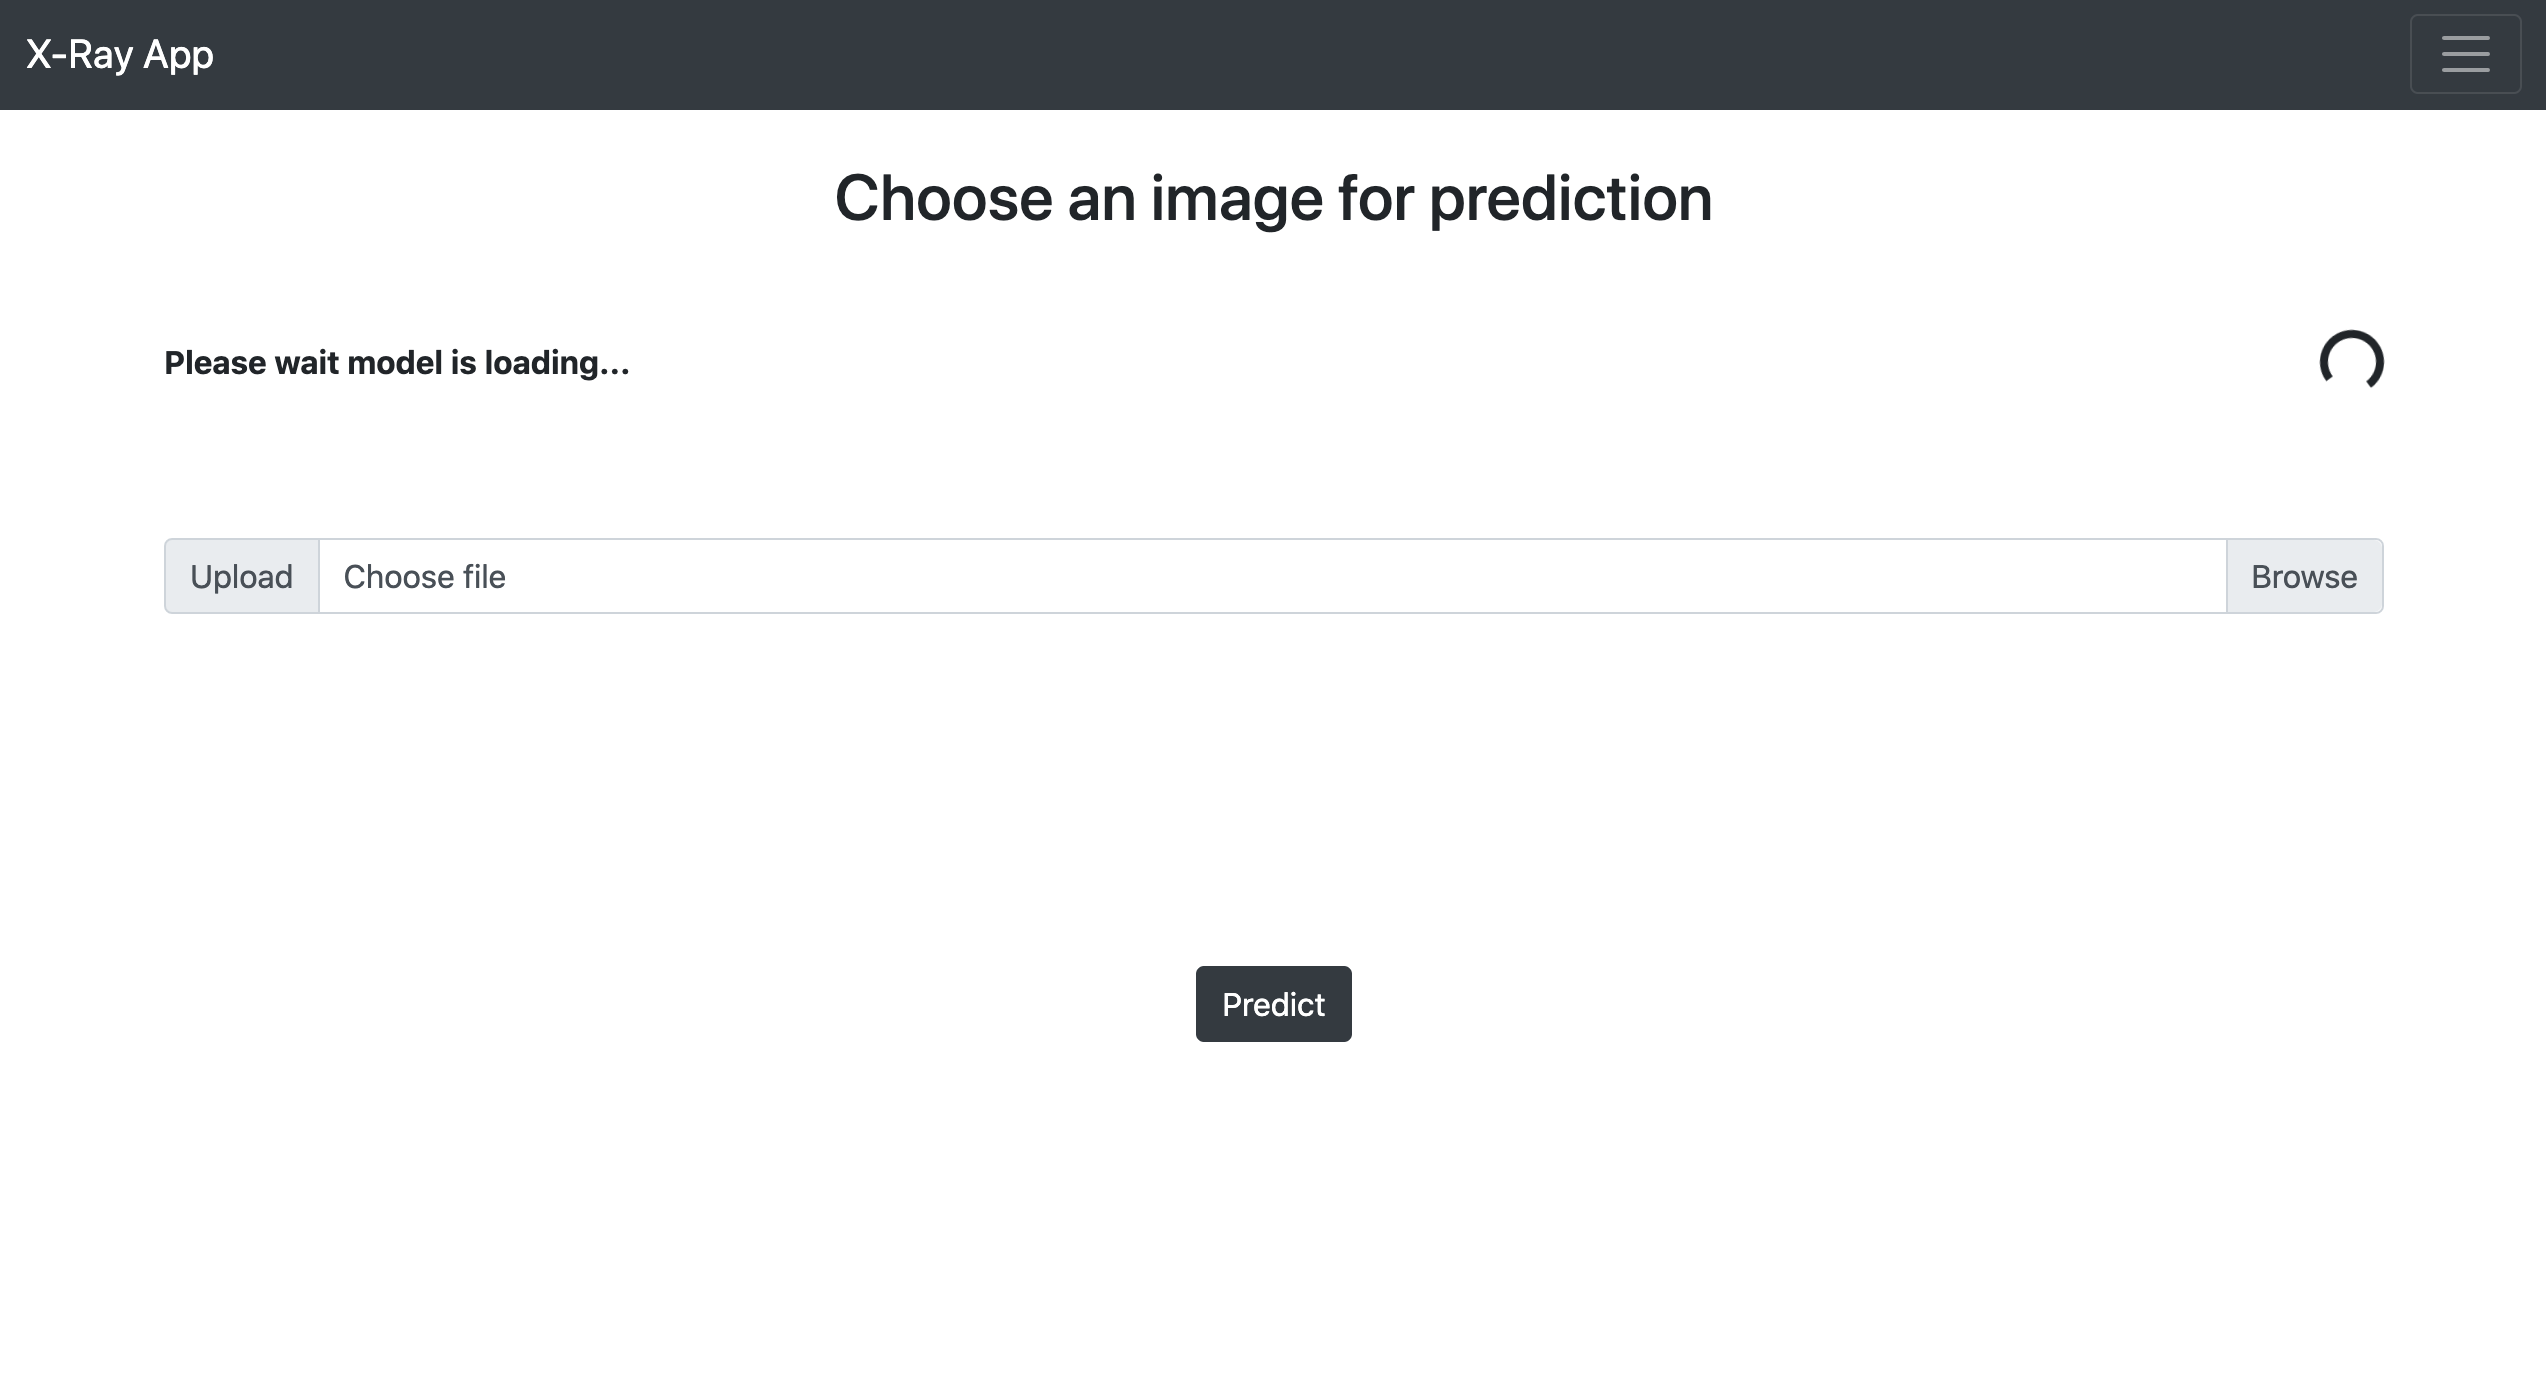
\includegraphics[width=\textwidth]{img/webhome.png}
    \caption{Main page for the deployment.}
    \label{fig:webhome}
\end{figure}

Because loading the model is required step that will take some time, loading of the model is started as soon as the user visiting the website and indicated to the user with spinner containing a message of the load process.
The spinner will be hidden upon completion of the model loading, indication that page ready for prediction.
At this point, user can select the X-ray image they want to run predictions which will get loaded to browser to insure user can verify the image.

\begin{figure}[H]
    \centering
    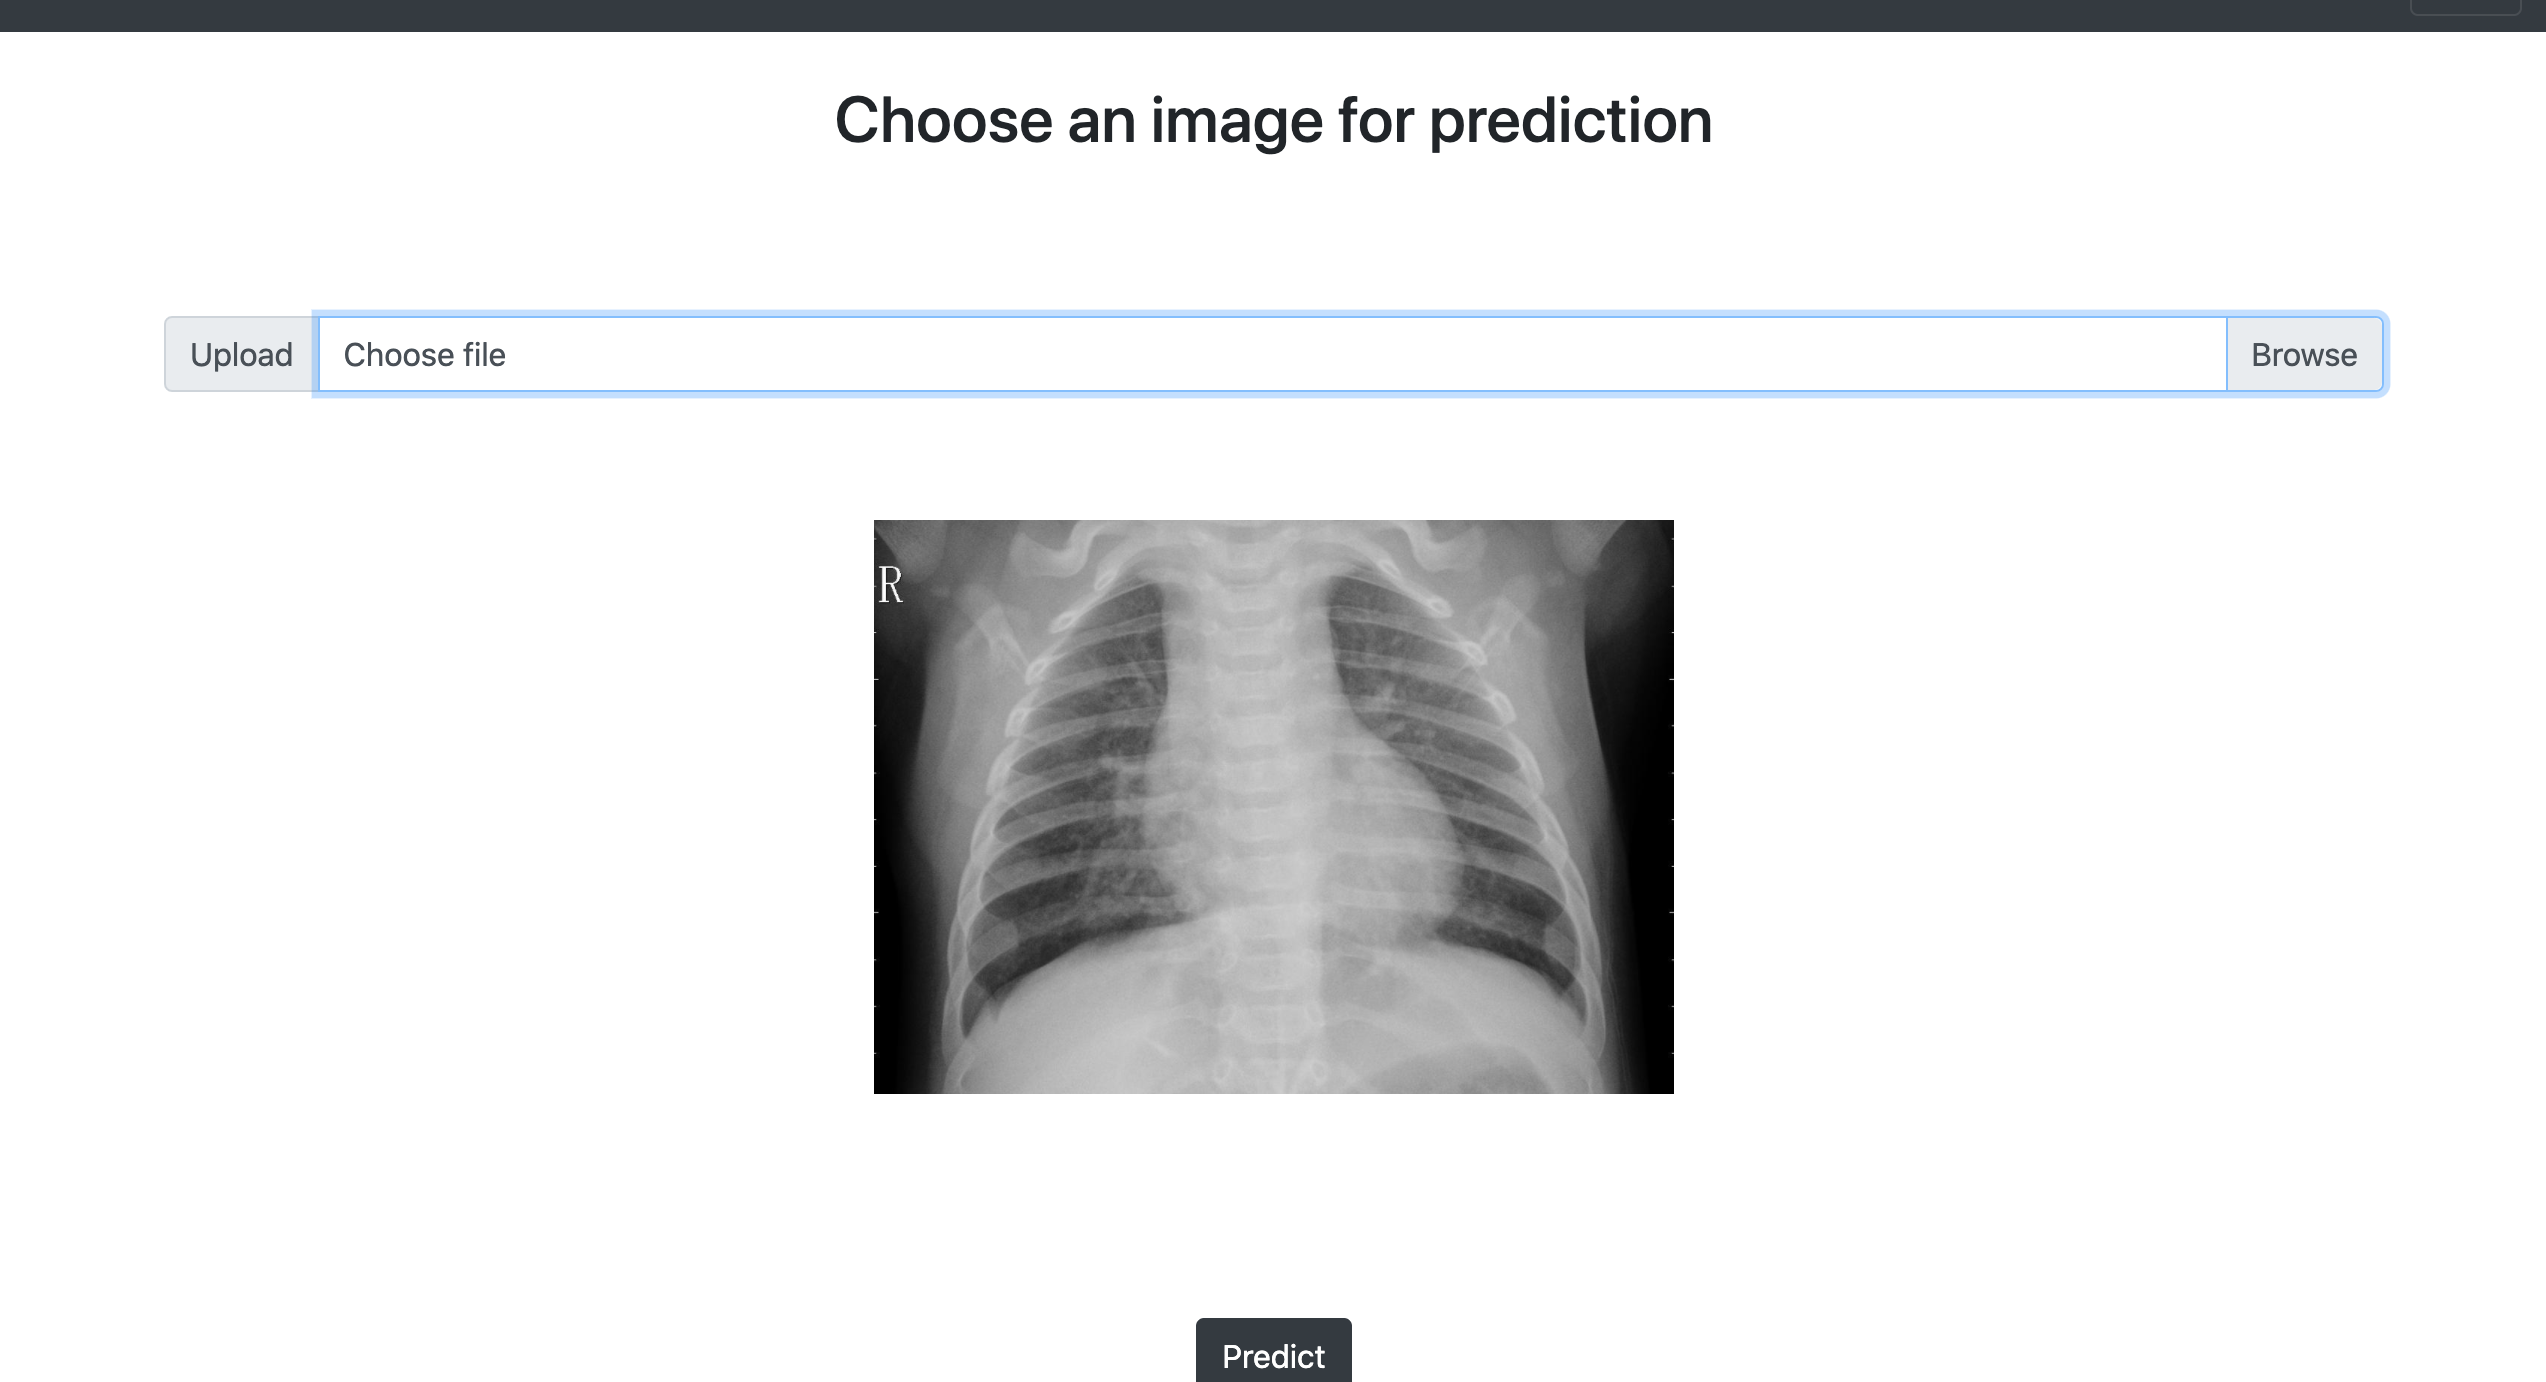
\includegraphics[width=\textwidth]{img/imageloaded.png}
    \caption{X-ray uploaded to website.}
    \label{fig:appimgload}
\end{figure}

At this point, user will click predict button and that action will trigger prediction function in JavaScript.
Background JavaScript code fetches the image loaded recently and with the help of build-in function turns the image to rank three tensor with RBG channels.
After acquiring the tensor from the image next steps are part of the feature engineering process.
Feature engineering in this app consists of resizing the image to expected dimensions by the model or in other words input shape of the model.
Immediately after that step reshaped image pixels have to be normalized to a maximum pixel value that puts tensor values between 0 to 1.
Final, because the original model is trained with batch data input data has to be a rank four tensor rather than three.
Achieving that is possible with a simple step that turning one image to batch data of one incident which commonly referred to as expanding the dimensionality.
Now that we have a right shaped tensor, predict method can be called on that image that returns a probability of image having class of \emph{true}, in this case, pneumonia.
In the final step, this probability will be translated into prediction by checking if the probability is less than or equal to 0.5 then the absence of pneumonia will be displayed otherwise prediction will be interpreted as the presence of pneumonia.
Product of the prediction then displayed on the web page to the end-user along with the probability value as shown below.

\begin{figure}[H]
    \centering
    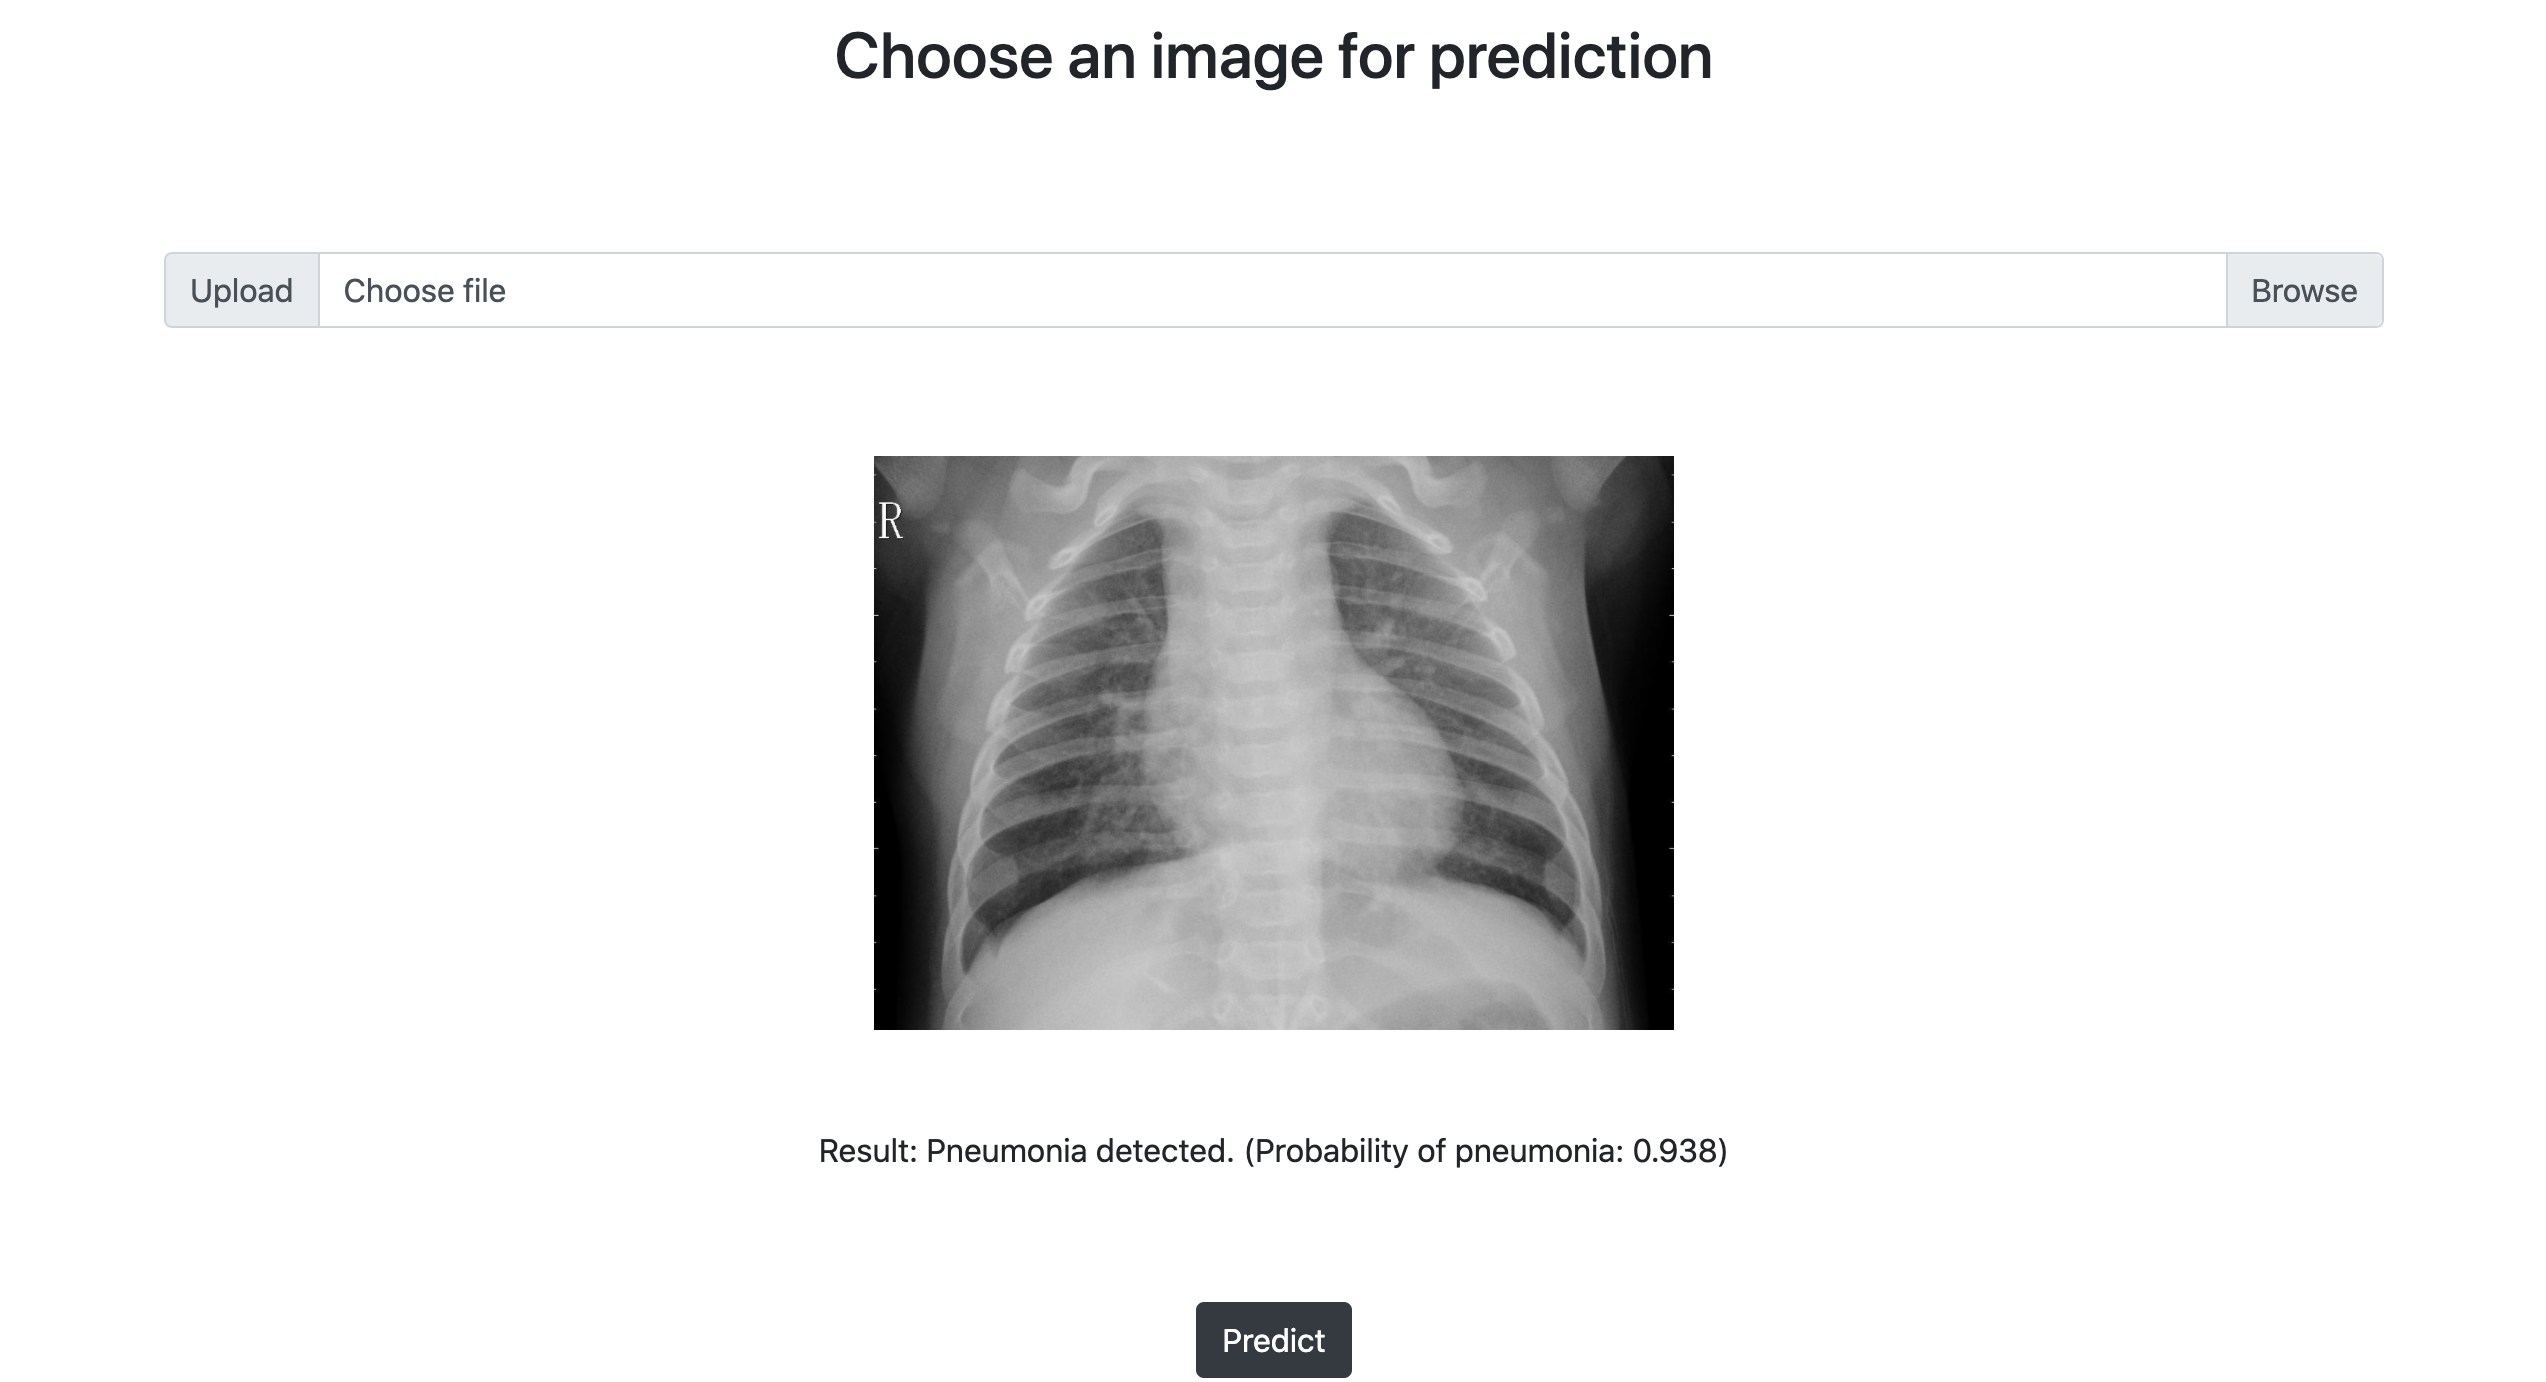
\includegraphics[width=\textwidth]{img/resultimg.png}
    \caption{Prediction results displayed to user.}
    \label{fig:appresult}
\end{figure}

% Why deployment
% why static webpage deployment
% pros of static web page
% - privacy
% - very little or no cost
% cons of static 
% - model is available to anyone
% - loading and processing times long

% Process of implementing my deployment
% webpage is served by GitHub
% image selected by user gets loaded and displayed in page
% Pre-processing
% - turn image to tensor
% - reshape tensor to desired size
% - normalize the tensor values
% - increase input dimension to batch of one

% returns prediction probability
% create a function to predict based on probability

\chapter{Conclusion}

\printbibliography[heading=bibintoc,
title={References}]
%\addcontentsline{toc}{chapter}{References}

\end{document}